\subsection{模的根}

定义 1. —— 设 A 是一个环。A-模 M 的根是定义为 M 的诸极大子模之交（VIII, 第 48 页，定义 2）的子模，或者等价地，是被从 M 到单 A-模的每个同态所零化的 M 的元素所成的集。

在本章的其余部分，我们把 A-模 M 的根记作 \(\mathfrak{R}_{\mathrm{A}}(\mathrm{M})\)，或简记作 \(\mathfrak{R}(\mathrm{M})\)。

设 A 是一个环。A-模 M 的根归结为 0（这时我们滥用语言称 M 是无根的），当且仅当存在单 A-模的一个族 \((\mathrm{S}_{i})_{i\in\mathrm{I}}\) 与 A-线性映射的一个族 \((f_{i})_{i\in\mathrm{I}}\)（\(f_{i}:M\to S_{i}\)），使得我们有 \(\cap_{i\in\mathrm{I}}\mathrm{Ker}(f_{i})=0\)。这等价于 M 同构于单 A-模的一个乘积的子模。

例. —— 1) 设 \(\mathfrak{a}\) 是 A 的一个左理想。A-模 \(\mathrm{A}_s / \mathfrak{a}\) 的根等于 \(\mathfrak{a}' / \mathfrak{a}\)，其中 \(\mathfrak{a}'\) 是 A 的包含 \(\mathfrak{a}\) 的诸极大左理想之交。特别地，Z-模 \(\mathbf{Z}\) 的根归结为 0，而 Z-模 \(\mathbf{Z} / p^n\mathbf{Z}\) 的根等于 \(p\mathbf{Z} / p^n\mathbf{Z}\)（对每个素数 \(p\) 与每个整数 \(n \geqslant 1\)）。

\begin{enumerate}
\def\labelenumi{\arabic{enumi})}
\setcounter{enumi}{1}
\tightlist
\item
  设 A 是一个不是体的主理想整环，K 是它的分式域。作为 K-模，K 是无根的。我们来证明把 K 看作 A-模时，其根等于 K；等价地，我们必须证明从 K 到单 A-模 S 的每个 A-线性映射 f 均为零。由 VII, §4, No.~8, 第 25 页，我们可以假设 S 等于 \(\mathrm{A}/(\pi)\)，其中 \(\pi\) 是 A 的一个不可约元。我们有 \(f(x) = f\left(\pi \frac{x}{\pi}\right) = \pi f\left(\frac{x}{\pi}\right) = 0\)（对每个 \(x \in \mathrm{K}\)），因为 \(\pi \mathrm{S} = 0\)。
\end{enumerate}

命题 1. —— 设 M 与 N 是 A-模，f 是从 M 到 N 的一个同态。我们有 \(f(\mathfrak{R}(M)) \subset \mathfrak{R}(N)\)，且若 f 是满射且 f 的核包含于 M 的根中，我们甚至有等式。

设 g 是从 N 到一个单 A-模的同态；于是 \(\mathfrak{R}(M)\) 包含于 \(g \circ f\) 的核，从而 \(f(\mathfrak{R}(M))\) 包含于 g 的核。于是我们有 \(f(\mathfrak{R}(M)) \subset \mathfrak{R}(N)\)。现在设 f 是满射且其核包含于 \(\mathfrak{R}(M)\)。设 y 是 \(\mathfrak{R}(N)\) 的一个元素，x 是 y 的逆像中的一个元素。若 g 是从 M 到单 A-模 S 的一个同态，则其核包含 M 的根，因而包含 f 的核。由于同态 f 是满射，存在从 N 到 S 的同态 h 使得 \(g = h \circ f\)。由于 \(y = f(x)\) 属于 \(\mathfrak{R}(N)\)，我们有 \(h(f(x)) = 0\)，即 \(g(x) = 0\)；于是 x 属于 \(\mathfrak{R}(M)\)，这就证明了包含关系 \(\mathfrak{R}(N) \subset f(\mathfrak{R}(M))\)。

推论 1. —— 设 M 是一个 A-模，N 是 M 的一个子模。

\begin{enumerate}
\def\labelenumi{\alph{enumi})}
\item
  我们有 \(\Re (\mathrm{N})\subset \Re (\mathrm{M})\cap \mathrm{N}.\)
\item
  我们有 \((\Re (\mathrm{M}) + \mathrm{N}) / \mathrm{N}\subset \Re (\mathrm{M} / \mathrm{N})\)。若 N 包含于 \(\Re (\mathrm{M})\)，则我们有等式 \(\Re (\mathrm{M} / \mathrm{N}) = \Re (\mathrm{M}) / \mathrm{N}\)
\item
  模 \(\mathrm{M} / \Re (\mathrm{M})\) 是无根的。若模 \(\mathrm{M} / \mathrm{N}\) 是无根的，则我们有 \(\Re (\mathrm{M})\subset \mathrm{N}\)。
\end{enumerate}

断言 a) 由把命题 1 应用于从 N 到 M 的典范单射得出，而断言 b) 由把命题 1 应用于从 M 到 M/N 的典范映射得出。由 b)，我们推出：若 \(N = \Re(M)\)，则 M/N 是无根的；若 M/N 是无根的，则我们有 \(\Re(M) \subset N\)。

\pandocbounded{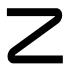
\includegraphics[keepaspectratio]{images/part001_4ea857d0.jpg}}

由例 1 可知，可能存在包含 \(\Re(\mathrm{M})\) 的子模 N，使得 M/N 的根不为零。

推论 2. —— 设 \((\mathrm{M}_{i})_{i\in\mathrm{I}}\) 是一个 A-模族，P 是它们的乘积，S 是它们的直和。我们有 \(\Re(\mathrm{P})\subset\prod_{i\in\mathrm{I}}\Re(\mathrm{M}_{i})\) 与 \(\Re(\mathrm{S})=\bigoplus_{i\in\mathrm{I}}\Re(\mathrm{M}_{i})\)。

对 \(i \in I\)，设 \(\pi_{i}\) 是从 P 到 \(M_{i}\) 的指标为 i 的投影。由命题 1，我们有 \(\pi_{i}(\mathfrak{R}(P)) \subset \mathfrak{R}(M_{i})\)（对每个 \(i \in I\)）；这就证明了第一个断言。我们有 \(S \subset P\)，因而

\[
\mathfrak {R} (S) \subset S \cap \mathfrak {R} (P) \subset S \cap \prod_ {i \in I} \mathfrak {R} (M _ {i}) = \bigoplus_ {i \in I} \mathfrak {R} (M _ {i}).
\]

此外，我们有 \(M_{i} \subset S\)，从而 \(\Re(M_{i}) \subset \Re(S)\)（对每个 \(i \in I\)），于是 \(\oplus_{i \in I} \Re(M_{i}) \subset \Re(S)\)。

存在一些模族，使得乘积的根不同构于诸根的乘积（VIII, 第 166 页，习题 3）。

命题 2. —— 设 M 是一个有限生成的 A-模。

\begin{enumerate}
\def\labelenumi{\alph{enumi})}
\item
  若 \(\mathbf{M}\) 不归结为 0，则我们有 \(\Re (\mathbf{M})\neq \mathbf{M}\)。
\item
  若 N 是 M 的一个子模，使得 \(\mathrm{N} + \Re(\mathrm{M}) = \mathrm{M}\)，则我们有 N = M。
\end{enumerate}

设 N 是 M 的一个真子模。由 VIII, 第 49 页的命题 3，存在 M 的一个包含 N 的极大子模 L。我们有 \(\mathrm{N} + \Re(\mathrm{M}) \subset \mathrm{L}\)，更必然有 \(\mathrm{N} + \Re(\mathrm{M}) \neq \mathrm{M}\)。这就证明了 b)；特例 N = 0 即给出断言 a)。

推论. —— 设 M 是一个 A-模，\((x_{i})_{i\in\mathbb{I}}\) 是 M 的一个生成族，x 是 M 的一个元素。下列性质等价：

\begin{enumerate}
\def\labelenumi{(\roman{enumi})}
\item
  我们有 \(x \in \Re(\mathbb{M})\)。
\item
  M 的每个使 \(\mathrm{N} + \mathrm{A}x = \mathrm{M}\) 的子模 N 都等于 M。
\item
  对 A 的元素的每个族 \((a_{i})_{i\in\mathrm{I}}\)，族 \((x_{i}+a_{i}x)_{i\in\mathrm{I}}\) 生成 A-模 M。
\item
  \(\Rightarrow\) (ii)：设 x 属于 \(\Re(\mathrm{M})\)。设 N 是 M 的一个子模，使得 \(N + Ax = M\)。我们有 \(N + \Re(M) = M\)；因而 A-模 M/N 等于它的根（命题 1 的推论 1, b)）。由于它是单生成的，它为零（命题 2），于是 M = N。
\item
  \(\Rightarrow\) (iii)：设 \((a_{i})_{i\in\mathrm{I}}\) 是 A 的元素的一个族。用 N 表示由族 \((x_{i}+a_{i}x)_{i\in\mathrm{I}}\) 生成的 M 的子模。我们有 \(x_{i}\in N+Ax\)（对每个 \(i\in I\)），因而 \(N+Ax=M\)。若性质 (ii) 成立，则 N 等于 M。
\item
  \(\Rightarrow\) (i)：设 x 不属于 \(\Re(\mathrm{M})\)。则存在 M 的一个不包含 x 的极大子模 N。由于 N 是极大的，我们有 \(N + Ax = M\)；因而每个元素 \(x_{i}\) 都可写成 \(y_{i} - a_{i}x\)，其中 \(y_{i} \in N\)，\(a_{i} \in A\)。族 \((x_{i} + a_{i}x)_{i \in I}\) 包含于 N，故不生成 M。
\end{enumerate}

命题 3. —— a) 半单模是无根的。

\begin{enumerate}
\def\labelenumi{\alph{enumi})}
\setcounter{enumi}{1}
\tightlist
\item
  一个模是半单的且有限生成的，当且仅当它是无根的且是阿廷的。
\end{enumerate}

按定义，单模的根归结为 0。若模 M 是半单的，则它是单子模的一个族 \((\mathrm{S}_{i})_{i\in\mathrm{I}}\) 的直和，且由上面命题 1 的推论 2，我们有 \(\mathfrak{R}(\mathrm{M})=\bigoplus_{i\in\mathrm{I}}\mathfrak{R}(\mathrm{S}_{i})\)，因而 \(\mathfrak{R}(\mathrm{M})=0\)。

此外，若 M 是有限生成的，则由 VIII, 第 71 页的命题 10，它是阿廷的。

反之，设 M 是阿廷的且无根的。把 VIII, 第 2 页应用于 M 的极大子模所成的集，存在 M 的极大子模的一个有限族 \((\mathrm{N}_{i})_{i\in\mathrm{I}}\)，其交归结为 0。于是 M 同构于 \(\bigoplus_{i\in\mathrm{I}}(\mathrm{M}/\mathrm{N}_{i})\) 的一个子模。因此，它是半单的且具有有限长度，更必然是有限生成的。

